\section{DNS}
In this section we make a full \gls{DNS} configuration. We describe every step. \newline First we install \textbf{unbound} , a DNS resolver which will be used from now for all DNS requests from this server.
\begin{lstlisting}
<INFO> - Tue Jan  8 11:15:22 UTC 2019 - Starting DNS Configurations.
*NOTE* We install two DNS Server, one for internal DNS requests (for this server and/or home clients) and one authoritative DNS Server for your domain
*PART 0: We install the basic configuration for unbound - we come back to it later
<INFO> - Tue Jan  8 11:15:22 UTC 2019 - Install DNS
<INFO> - Tue Jan  8 11:15:24 UTC 2019 - Will install 'unbound' now. Please wait...
............
<INFO> - Tue Jan  8 11:15:36 UTC 2019 - Package 'unbound' is installed now.
<INFO> - Tue Jan  8 11:15:37 UTC 2019 - Configure DNS Hardening (Hide version, use root-hints file, use trust-anchored zones for DNSSEC requests)
<INFO> - Tue Jan  8 11:15:37 UTC 2019 - Configure DNS Ports, IPs
<INFO> - Tue Jan  8 11:15:37 UTC 2019 - Server will listen with localhost on port 53
<INFO> - Tue Jan  8 11:15:37 UTC 2019 - Configure DNS Access
<INFO> - Tue Jan  8 11:15:37 UTC 2019 - Configure this Client
<INFO> - Tue Jan  8 11:15:37 UTC 2019 - Server will use localhost as DNS
\end{lstlisting}

After we continue with the \textbf{authoritative Name Server: NSD}, have ready your domain (highlighted).
\begin{lstlisting}[escapeinside=||]
*PART 1: We start with the authoritative Name Server: NSD

!!CAUTION!! you need your own domain - IF NOT the server wont be functional
DO NOT use a domain which does not belong to you, it may be illegal
*NOTE* If you want to test it only, you can get a free domain like .tk or .ga - just search in your favorite web search engine (duckduckgo, google etc..)

Press enter to continue

 *** QUESTION *** do you have your own domain? (y/n/abort) |\colorbox{yellow}{y}|
<INFO> - Tue Jan  8 11:15:59 UTC 2019 -

 *** QUESTION *** please enter your domain:   |\colorbox{yellow}{examplerun.cf}|

 *** QUESTION *** is examplerun.cf correct? (y/n/abort)   |\colorbox{yellow}{y}|
 
 <INFO> - Tue Jan  8 11:16:15 UTC 2019 - We will configure the authoritative DNS Server with the domain: |\colorbox{yellow}{examplerun.cf}|
 \end{lstlisting}

 Once the domain is set, check if the follow output is your extern IP, if yes continue.
\begin{lstlisting}[escapeinside=||]
 *** QUESTION *** is this |\colorbox{yellow}{104.248.137.212}| your external IP address ? (y (default)/n/abort)   |\colorbox{yellow}{y}|
<INFO> - Tue Jan  8 11:16:48 UTC 2019 - We will configure the authoritative DNS Server with this: |\colorbox{yellow}{104.248.137.212}|
<INFO> - Tue Jan  8 11:16:48 UTC 2019 - Install authoritative DNS for : |\colorbox{yellow}{examplerun.cf}|
<INFO> - Tue Jan  8 11:16:48 UTC 2019 - Will install 'nsd' now. Please wait...
..........
<INFO> - Tue Jan  8 11:16:57 UTC 2019 - Package 'nsd' is installed now.
<INFO> - Tue Jan  8 11:16:59 UTC 2019 - Will install 'ldnsutils' now. Please wait...
........
<INFO> - Tue Jan  8 11:17:06 UTC 2019 - Package 'ldnsutils' is installed now.
<INFO> - Tue Jan  8 11:17:06 UTC 2019 - Configure NSD
<INFO> - Tue Jan  8 11:17:06 UTC 2019 - Configure Forward Zone
<INFO> - Tue Jan  8 11:17:06 UTC 2019 - Configure Backward Zone
<INFO> - Tue Jan  8 11:17:06 UTC 2019 - Final steps
<INFO> - Tue Jan  8 11:17:11 UTC 2019 - Test NSD
\end{lstlisting}

Now you can change, as described, your domain (\gls{Glue Records}). 
\begin{lstlisting}[escapeinside=||]
PART 2: You have a full functional authoritative Name Server BUT your domain hoster does not know it!
 !! VERY IMPORTANT !! GO to your domain hoster, change the name server for your domain to :
                |\colorbox{yellow}{ns1.examplerun.cf with IP: 104.248.137.212}|
                |\colorbox{yellow}{ns2.examplerun.cf with IP: 104.248.137.212}|
 !! VERY IMPORTANT !! DO the same for the |\colorbox{yellow}{Glue Records}|, with the same name server and IPs
NOTE: It may take some time to change it - if you have difficulties with this part use your favorite web search engine

If you are done, press enter to continue
\end{lstlisting}

In the last part, if you use the server in your home/work network you can make the domain resolver we installed (unbound) accessible for your local clients. Mostly it is not the case so you can continue with ``enter''. At the end we test to resolve a \textbf{ipv4} and a  \textbf{ipv6} address. 
\begin{lstlisting}[escapeinside=||]
PART 3: *** QUESTION *** Do you rent this server or is it in your internal network area? If you dont know what it means just press enter. (intern / <enter> (default))  |\colorbox{yellow}{\textless enter\textgreater}|
<INFO> - Tue Jan  8 11:17:40 UTC 2019 - Test local DNS
<INFO> - Tue Jan  8 11:17:40 UTC 2019 - |\colorbox{yellow}{Test ipv4 address}|
www.google.com.         3600    IN      A       216.58.210.4
<INFO> - Tue Jan  8 11:17:40 UTC 2019 - |\colorbox{yellow}{Test ipv6 address}|
ipv6.google.com.        604800  IN      CNAME   ipv6.l.google.com.
ipv6.l.google.com.      3600    IN      AAAA    2a00:1450:4005:800::200e

Successfully installed NSD and Unbound
\end{lstlisting}
And we are done with the DNS part!
\newpage

\subsection{DNS architecture diagram}
For a better understanding of how a domain name will be resolved, here is a small diagram which indicates how those two servers are separated.
\begin{figure}[H]
	\centering
	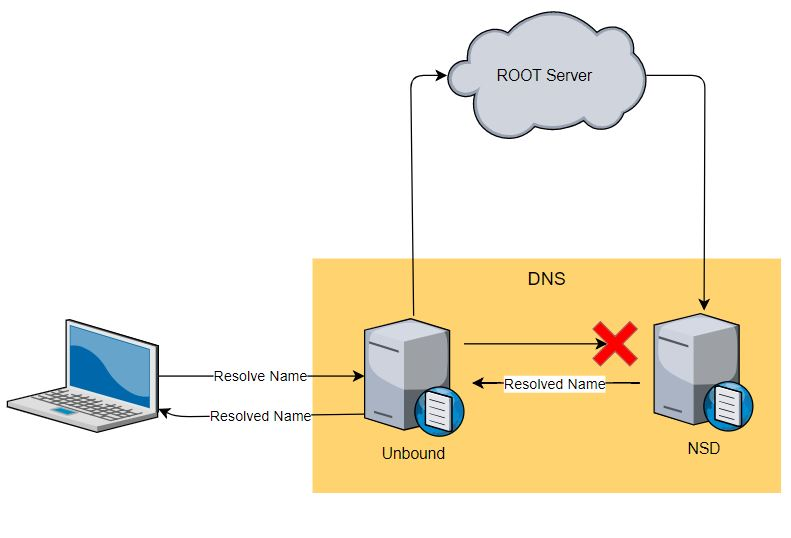
\includegraphics[width=0.9\linewidth]{diagram/dns_arch_diagramm.JPG}
	\caption{Architecture DNS}
	\label{fig:beforeWeb}
\end{figure}
\newpage
\subsection{DNS process diagram}
Here we have process diagram of how the script works with all possible outcomes.

\begin{figure}[H]
	\usetikzlibrary{shapes,arrows,calc}
	\centering
	\includestandalone[scale=0.9]{diagram/process_diagramm_DNS}
	\caption{DNS process diagram}
\end{figure}

\subsection{Multiple domains}
After installation you can use multiple sub domains of your domain. All domains will be resolved, as it is configured with a \gls{wild-card}: (in this example) *.examplerun.cf. As the script was designed for someone with basic understanding of computer technology, to have multiple domains on the same server is not possible.

\newpage
